\chapter[Détail du code]{Détail du code}

\textit{Pour faciliter l'écriture et la compréhension du code, on utilise la méthode Modèle/Vue/Contrôleur. Dans cette section, on détaillera donc les différentes fonctions implémentées en suivant ce modèle.}

\section{Partie Vue}

La partie Vue contient le code relatif à l'interface graphique. Après la réalisation des trois interfaces graphiques avec QtDesigner, l'utilitaire PyUic5 a permis de transcrire le code C++ en langage Python. \\

\noindent Trois fichiers ont alors été créés et définissent les trois classes :
\begin{itemize}[label=$\rightarrow$]
	\item La classe \textit{Ui\_InterfacePrincipale} du fichier \textit{classificationActive.py} comporte le code de l'interface principale. Elle définit les caractéristiques des boutons, des labels de texte et de la fenêtre graphique dans une première méthode \textit{setupui} : ce sont les attributs de l'interface. Une méthode \textit{retranslateUi} permet de mettre à jour le texte des attributs.\\
	\item La classe \textit{Ui\_ChargementFichiers} du fichier \textit{chargementFichiers.py} comporte le code de l'interface de chargement. Elle dispose elle aussi des deux méthodes \textit{setupui} et \textit{retranslateUi}. Pour permettre l'affichage des différentes stratégies dans le menu déroulant, on utilise la variable globale STRATEGIES définie dans le fichier \textit{strategy.py}. Ainsi, ce menu sera mis à jours automatiquement en cas d'implémentation d'une nouvelle stratégie.\\
	\item La classe \textit{Ui\_ChoixClasse} du fichier \textit{choixClasse.py} comporte le code de l'interface de sélection d'une nouvelle classe. Elle dispose des méthodes \textit{setupui} et \textit{retranslateUi}.\\
\end{itemize}

En cas de modification de l'interface, ces fichiers sont réécrits, mais cela n'impactera pas le code du programme principal. Une seule modification doit être apportée à ces codes générés automatiquement : il faut modifier le chemin de l'image du point d'interrogation. En effet, ce chemin est contenu dans un fichier ressource en C++, qui n'est pas traduisible simplement en Python avec PyUic5. 

\newpage

\section{Partie Modèle}

La partie Modèle contient l'organisation des données. Ainsi, trois nouveaux fichiers viennent définir trois classes : la classe \textit{Building}, la classe \textit{Background} et la classe \textit{Strategy}.

\subsection{La classe \textit{Building}}

\begin{figure}[!h]
	\begin{minipage}{0.55\linewidth}\parindent12pt
		\indent La classe \textit{Building} est codée dans le fichier \textit{building.py}. Un objet de type \textit{Building} est défini par 4 attributs : identity (identifiant de l'objet), geometry, classe et probability. \\
	\end{minipage}
	\hfill
	\begin{minipage}{0.45\linewidth}
		\centering
		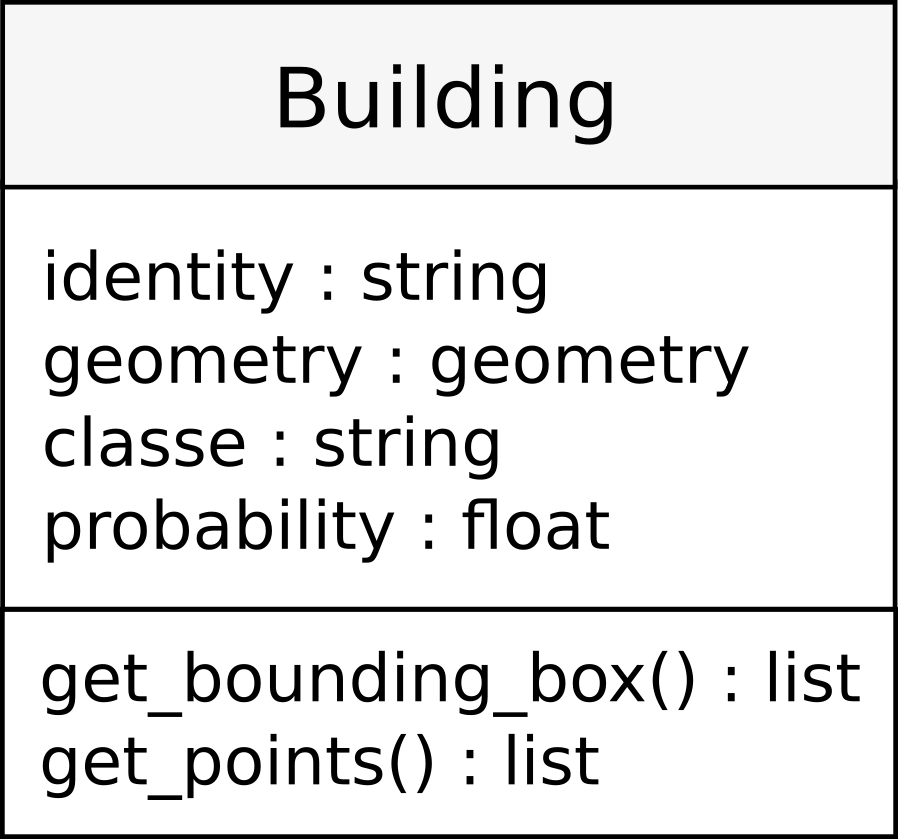
\includegraphics[scale=0.40]{building_classe.png}  \\
		\caption[Classe \textit{Building}]{Classe \textit{Building}}
		\label{fig:classebuilgind}
	\end{minipage}
\end{figure}

\noindent Deux méthodes lui sont associées : 
\begin{itemize}[label=$\rightarrow$]
	\item \textit{get\_points} retourne la liste de tous les sommets de chaque géométrie de l'entité. Ainsi, si une entité est composée de 3 triangles, la liste de sortie contiendra 9 points. Chaque point est codé par un couple de coordonnées (x,y).
	\item \textit{get\_bounding\_box} parcourt l'ensemble des coordonnées x et y d'une liste et retourne les valeurs maximales et minimales de ces deux paramètres. Cela permet de définir la fenêtre d'emprise d'une entité.
\end{itemize}

\noindent Le fichier \textit{building.py} contient aussi deux fonctions :
\begin{itemize}[label=$\rightarrow$]
	\item \textit{read\_building} permet de construire des objets de type \textit{Building}. Elle prend comme paramètres d'entrée le dossier contenant les géométries (directory), l'identifiant, la classe et la probabilité d'une entité (building\_id, classe, probability). Elle retourne un objet de type \textit{Building}. La géométrie est construite en appelant la fonction \textit{get\_geometry}.
	\item \textit{get\_geometry} retourne les sommets des polygones contenus dans un fichier .SHP. Elle prend comme paramètres d'entrée le chemin du fichier .SHP, et renvoie une liste de tuples. Pour lire les formes contenues dans la géométrie, on utilise le module \textit{shapefile}.\\
\end{itemize}

\subsection{La classe \textit{Background}}

\begin{figure}[!h]
	\begin{minipage}{0.55\linewidth}\parindent12pt
		\indent La classe \textit{Background} est codée dans le fichier \textit{background.py}. Un objet de type \textit{Background} est défini par 3 attributs : reference\_point (coordonnées origines de l'image), pixel\_size (taille des pixels de l'image) et image (matrice d'image).\\
	\end{minipage}
	\hfill
	\begin{minipage}{0.45\linewidth}
		\centering
		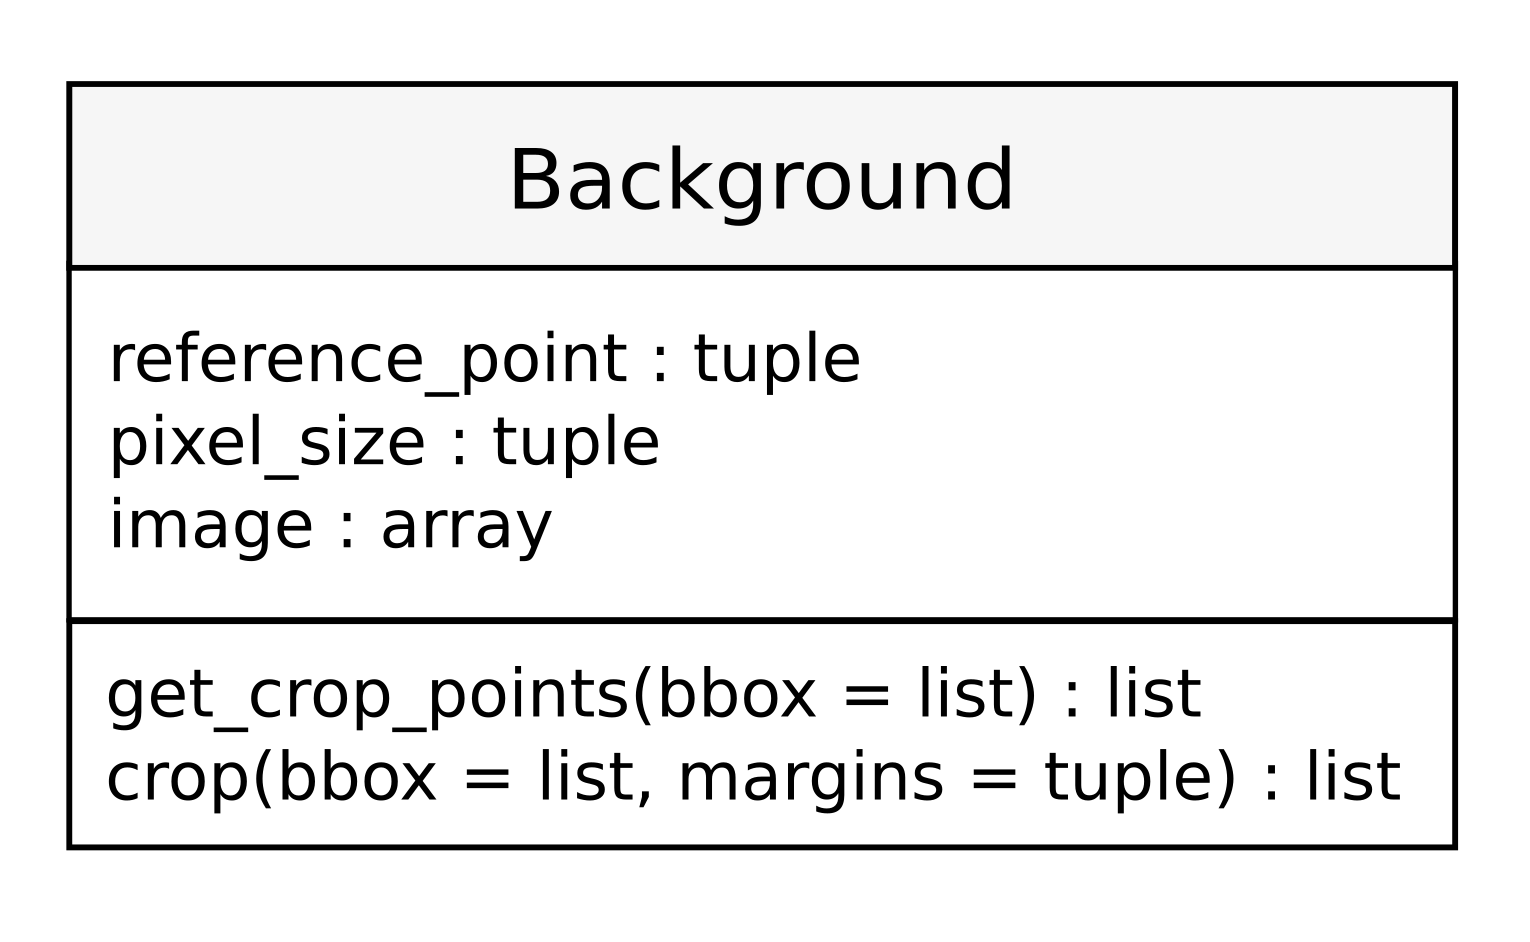
\includegraphics[scale=0.40]{background_classe.png}  \\
		\caption[Classe \textit{Background}]{Classe \textit{Background}}
		\label{fig:classeback}
	\end{minipage}
\end{figure}

\noindent Deux méthodes lui sont associées : 
\begin{itemize}[label=$\rightarrow$]
	\item \textit{get\_crop\_points} renvoie les extrémités de la fenêtre de rognage de l'orthoimage. Avec cette fonction, les extrémités de la fenêtre de rognage, exprimées dans un système métrique (= paramètre bbox), sont transformées en coordonnées pixels. 
	\item \textit{crop} est la fonction permettant de rogner une image. Elle prend en paramètres les extrémités de la fenêtre de rognage et les valeurs des marges. Pour chaque bande de l'orthoimage, on sélectionne la sous-matrice correspondant aux limites fixées. 
\end{itemize}

\noindent Le fichier \textit{building.py} contient aussi une fonction :
\begin{itemize}[label=$\rightarrow$]
	\item \textit{read\_background} permet de construire des objets de type \textit{Background}. Elle prend comme paramètre d'entrée le chemin de l'orthoimage (filename). La lecture de l'image utilise le package \textit{gdal} et ses méthodes associées. La fonction retourne un objet \textit{Background}, dont l'image associée est composée de 3 bandes.
\end{itemize}

\subsection{La classe \textit{Strategy}}

\indent Le fichier \textit{strategy.py} définit les classes correspondant aux stratégies de sélection des entités. A ce jour, seules deux méthodes ont été implémentées.\\

\begin{figure}[!h]
	\begin{minipage}{0.58\linewidth}\parindent12pt
		\noindent Le fichier définit donc trois classes :
		\begin{itemize}[label=$\rightarrow$]
			\item La classe \textit{Strategy} est la classe mère. Elle n'a pas d'attributs, mais elle définit une méthode \textit{filtre} qui prend une liste en paramètre mais ne retourne rien.
			\item La classe  \textit{Naive} est une classe fille, qui hérite des propriétés de la classe \textit{Strategy}. Elle n'a pas d'attributs, et sa méthode \textit{filtre}  retourne la liste donnée en paramètre sans aucune modification.
			\item La classe \textit{Random} est une classe fille, qui hérite des propriétés de la classe \textit{Strategy}. Elle prend comme attribut le nombre d'entité à retourner (\textit{selection\_number}). Sa méthode \textit{filtre} retourne un nombre fixé d'entités, aléatoirement sélectionnées dans la liste donnée en paramètre.\\
		\end{itemize}
	\end{minipage}
	\hfill
	\begin{minipage}{0.40\linewidth}
		\centering
		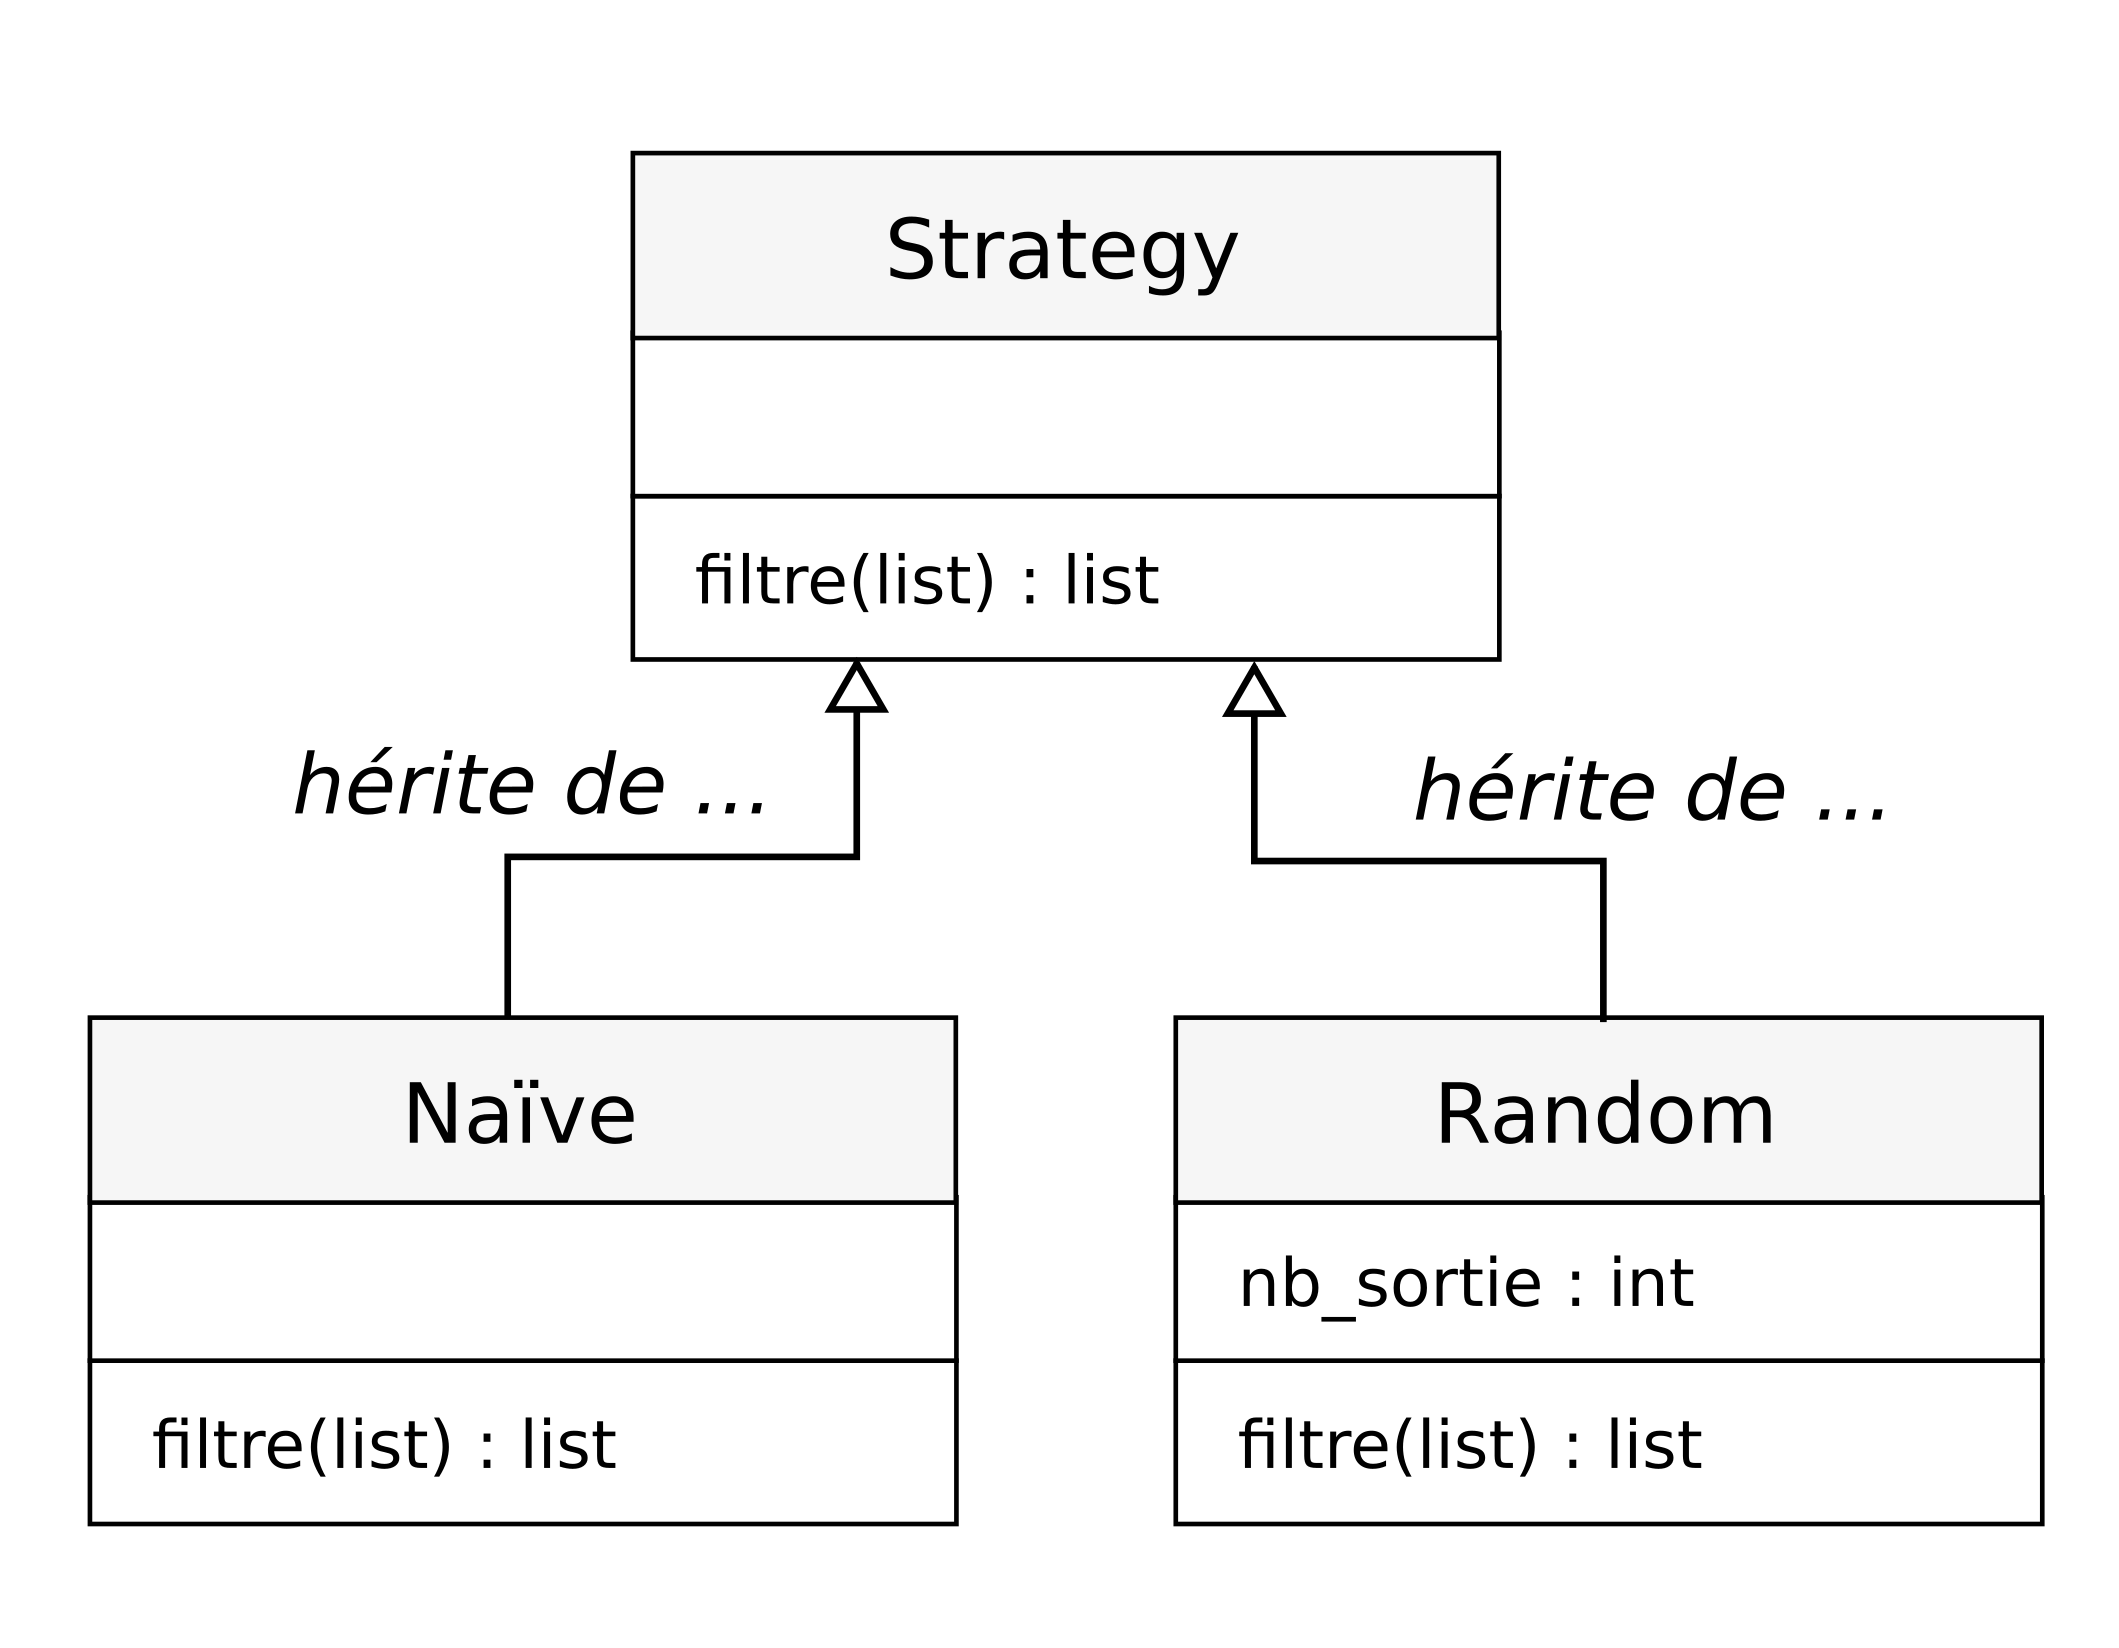
\includegraphics[scale=0.35]{classes_strategy.png}  \\
		\caption[Classe \textit{Background}]{Classe \textit{Background}}
		\label{fig:classestrat}
	\end{minipage}
\end{figure}

Ce fichier définit également une variable globale \textit{STRATEGIES}. Sous forme de dictionnaire, cette variable regroupe l'ensemble des classes filles de \textit{Strategy}. Ainsi, les clés du dictionnaire correspondent aux différentes classes stratégies. Les valeurs associées aux clés renseignent les attributs de la classe et les paramètres de la fonction filtre. Cette variable est créée en utilisant la réflexion, c'est à dire la capacité de Python à examiner ses propres structures internes. 

\section{Partie Contrôleur}

La partie Contrôleur contient les définitions informatiques des actions effectuées par l'utilisateur dans l'interface. Ces actions viennent modifier les données contenues dans le modèle, ce qui entraine un changement dans la vue.\\

La partie Contrôleur est codée dans le fichier \textit{interface.py}. Les trois classes définies dans ce document héritent des classes de la partie Vue. Ainsi, il est possible de définir les connexions entre les interfaces et les fonctions.

\begin{figure}[H]
	\centering
	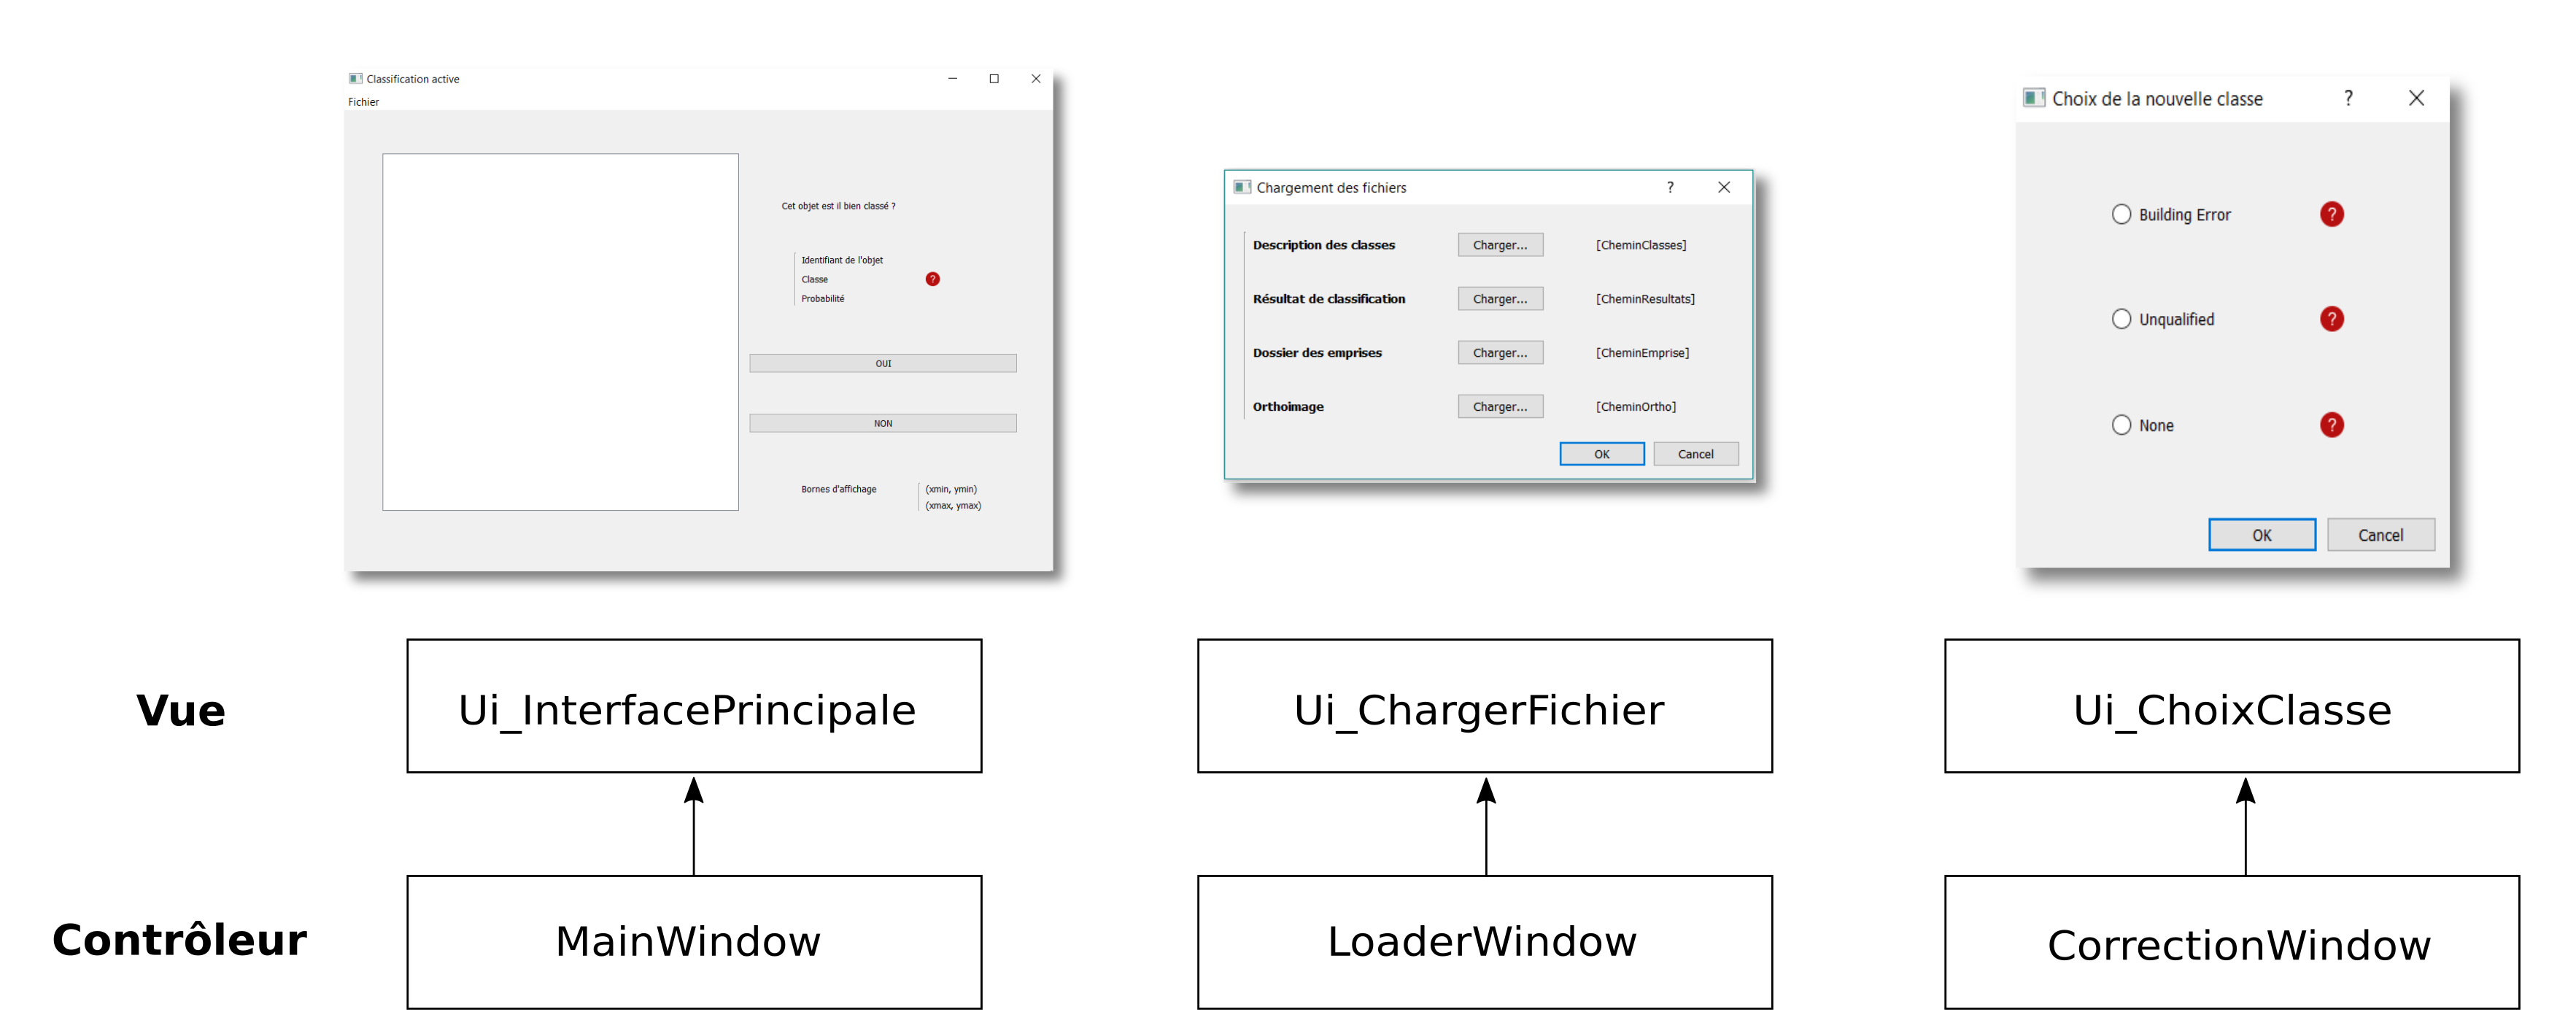
\includegraphics[scale=0.55]{Classes_interface.png}  \\
	\caption[Organisation des interfaces et héritages associés]{Organisation des interfaces et héritages associés}
	\label{fig:classesinterf}
\end{figure}

\subsection{Classe \textit{LoaderWindow}}

La classe \textit{LoaderWindow} hérite de la classe \textit{Ui\_ChargerFichier}. Elle définit et gère toutes les connexions de l'interface de chargement. Ses principaux attributs enregistrent les chemins d'accès des fichiers et les paramètres de traitement définis par l'utilisateur.\\

\noindent On distingue donc 7 méthodes pour cette classe :
\begin{itemize}[label=$\rightarrow$]
	\item \textit{select\_classes} est appelée lorsque l'utilisateur clic sur le premier bouton \textit{Charger}. Un objet QFileDialog est appelé et permet à l'utilisateur de sélectionner le fichier des classes. Si le chemin choisi est correct, il s'affiche dans le QLabel associé.
	\item \textit{select\_results} est appelée lorsque l'utilisateur clic sur le deuxième bouton \textit{Charger}. La fonction demande à l'utilisateur le chemin du fichier des résultats et l'affiche dans un label.
	\item \textit{select\_background} est appelée lorsque l'utilisateur clic sur le dernier bouton \textit{Charger}. La fonction demande à l'utilisateur le chemin de l'orthoimage et l'affiche dans un label.
	\item \textit{select\_building\_dir} est appelée lorsque l'utilisateur clic sur le troisième bouton \textit{Charger}. La fonction demande à l'utilisateur le chemin du dossier des emprises et l'affiche dans un label.
	\item \textit{current\_strategy} retourne la méthode de filtrage à utiliser en fonction du choix du menu déroulant (= comboBox). Cette fonction prend en paramètre d'entrée une liste d'entités, et retourne la liste filtrée.
	\item \textit{param\_strategy} met à jour l'affichage selon la valeur sélectionnée dans le menu déroulant (= comboBox). Ainsi, selon la stratégie sélectionnée, des parties de l'interface seront grisées ou dégrisées.
	\item \textit{get\_margins} retourne un tuple contenant les valeurs des marges rentrées par l'utilisateur.\\
\end{itemize}

\subsection{Classe \textit{MainWindow}}

La classe \textit{MainWindow} hérite de la classe \textit{Ui\_InterfacePrincipale}. Elle définit et gère toutes les connexions de l'interface principale. Elle possède de nombreux attributs et des méthodes qui utilisent et modifient ces attributs.\\
\newpage

\noindent On distingue donc 7 méthodes pour cette classe :
\begin{itemize}[label=$\rightarrow$]
	\item \textit{show\_loading\_window} est une méthode qui se lance lorsque l'utilisateur clic sur l'onglet \textit{Fichier > Charger ...}. La fenêtre de chargement des fichiers est appelée et l'utilisateur peut renseigner les chemins d'accès et les paramètres de traitement. Si tous les chemins sont renseignés, la fonction crée les variables nécessaires au traitement : le dictionnaire des classes (\textit{classes}) et la liste des résultats de l'auto-qualification (\textit{results}). Les résultats sont filtrés avec la fonction \textit{current\_strategy}, et une liste d'objets \textit{Building} est créée (variable \textit{input\_building}). Après avoir chargé l'orthoimage (méthode \textit{read\_background} de \textit{Background}), la phase d'affichage et d'interaction est lancée en appelant la méthode \textit{next}.
	\item \textit{next} est une méthode qui va tester la longueur de la liste \textit{input\_building}. S'il reste des éléments, elle enregistre et enlève le dernier élément de la liste (méthode \textit{pop}) et lance la fonction d'affichage. S'il n'y a plus d'éléments à présenter, la fonction \textit{save} est lancée puis le programme est fermé.
	\item \textit{show\_building} est une méthode permettant d'afficher un objet \textit{Building}. Elle initie l'affichage graphique en créant une \textit{scene}, puis y ajoute l'orthoimage rognée (méthode \textit{addPixmap}) et la géométrie (méthode \textit{addPolygon}). La mise à l'échelle de la scène est réalisée avec la méthode \textit{fitInView}. Les caractéristiques de l'entité sont affichées dans les différents labels (méthode \textit{setText}), ainsi que les bornes d'affichage. La méthode \textit{setToolTip} permet d'afficher des info-bulles.
	\item \textit{validate} permet de valider l'entité en cours de visualisation. Sa probabilité est modifiée et l'objet \textit{Building} est ajouté à la liste des résultats de sortie \textit{output\_building}. 
	\item \textit{correct} permet de corriger l'entité en cours de visualisation. La fenêtre de choix d'une nouvelle classe est appelée, et sa nouvelle valeur est enregistrée. La probabilité est modifiée et l'objet \textit{Building} est ajouté à la liste des résultats de sortie \textit{output\_building}.
	\item \textit{show\_correction\_window} est une méthode qui se lance lorsque l'utilisateur invalide le choix de la classe. La fenêtre de sélection d'une nouvelle classe est appelée et l'utilisateur peut sélectionner la nouvelle classe, qui est sauvegardée dans une variable \textit{new\_label}.
	\item \textit{save} permet à l'utilisateur de sélectionner le chemin d'enregistrement de son fichier. Si ce chemin est correct, un fichier .CSV est créé avec les données contenues dans la liste \textit{output\_building}. Si le chemin n'est pas valide, un message d'erreur est affiché.\\
\end{itemize}

La fonction \textit{show\_main\_window} est également définie dans le fichier \textit{interface.py}. Elle contient le code pour lancer l'affichage de l'interface principale. C'est cette fonction qui est appelée au lancement du programme.

\subsection{Classe \textit{CorrectionWindow}}

La classe \textit{CorrectionWindow} hérite de la classe \textit{Ui\_ChoixClasse}. Elle définit et gère toutes les connexions de l'interface de sélection d'une nouvelle classe.\\

\noindent On distingue deux méthodes pour cette classe :
\begin{itemize} [label=$\rightarrow$]
	\item \textit{check} met à jour la valeur des labels selon la classe de l'entité en cours de visualisation. En effet, les nouveaux choix proposés à l'utilisateur sont des classes différentes de celle affichée dans l'interface principale.
	\item \textit{new\_choice} teste le bouton coché par l'utilisateur, et retourne la valeur du label associé. Cela permet d'enregistrer la nouvelle classe choisie par l'utilisateur.
\end{itemize}

